\documentclass[10pt]{beamer}


\usetheme{metropolis}
\usepackage{appendixnumberbeamer}


\usepackage{booktabs}
\usepackage[scale=2]{ccicons}

\usepackage{pgfplots}
\usepgfplotslibrary{dateplot}

\usepackage{xspace}
\newcommand{\themename}{\textbf{\textsc{metropolis}}\xspace}


\usepackage{graphicx} % http://ctan.org/pkg/graphicx (don't use 'demo' in your document)
\usepackage{xcolor}
\usepackage{adjustbox}
\usepackage{graphicx}

\usepackage[utf8]{inputenc}

% REMOVE PAGE NUMERING:
\setbeamertemplate{footline}[frame number]{} % gets rid of bottom navigation bars
\setbeamertemplate{navigation symbols}{}  % gets rid of bottom navigation symbols
\setbeamertemplate{footline}{}  % gets rid of footer
%will override 'frame number' instruction above
%comment out to revert to previous/default definitions	

\title{Regularisierung von linearer Regression}
\date{}
\author{Philipp Grafendorfer, Michael Kastner, Raphael Peer}



\begin{document}

\setbeamerfont{frametitle}{size=\Large}
\setbeamertemplate{frametitle}[default][center]

\maketitle

\section{Daten}


\begin{frame}{Ames House price Dataset}
	
	\begin{Large}
		Datensatz:
	\end{Large}
	\begin{itemize}
		\item 1460 Häuser
		\item 79 erklärende Variablen (numerisch und kategorisch)
		\item bekannter Übungsdatensatz
	\end{itemize}
	
	\begin{Tiny}		
		Quelle: \url{https://www.kaggle.com/c/house-prices-advanced-regression-techniques}
	\end{Tiny}
\end{frame}


\begin{frame}{Fehlende Werte: Übersicht}
	
	\begin{figure}
		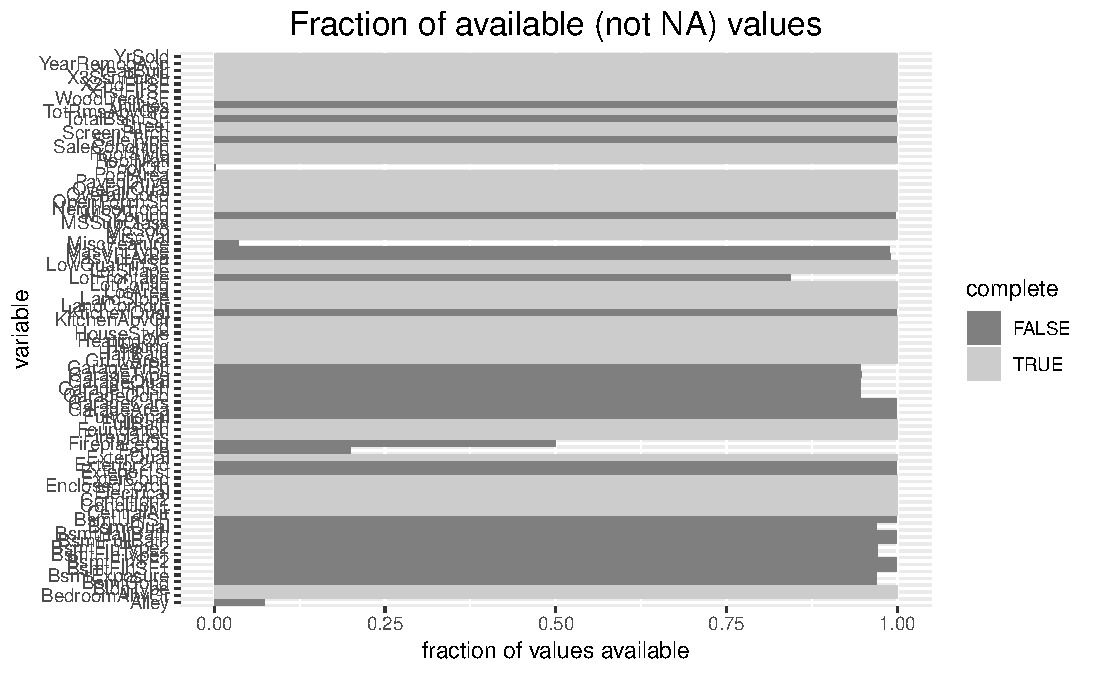
\includegraphics[width=\textwidth, keepaspectratio]{figures/na_stats}
	\end{figure}
	
\end{frame}

\begin{frame}{Fehlende Werte: Strategie}
	
	\begin{Large}{Umgang mit fehlenden Werten:}\end{Large}
	\begin{itemize}
		\item Bei mehr als 10\% Fehlenden Werten: Variable verworfen
		\item Bei numerischen Variablen: NA durch Median der Variable ersetzt
		\item Bei kategorischen Variablen: NA als eigene Kategorie (Kategorie 'unbekannt')
	\end{itemize}
	
\end{frame}

\begin{frame}{Problem mit validation-set: seltene Factor-levels}
	\begin{columns}[T,onlytextwidth]
		
		\column{0.5\textwidth}
		\metroset{block=fill}
		
		\begin{block}{data-frame}
			einige levels im validation-set aber nicht im trainings-set\\
			$\implies$ unbekannte dummy Variablen im validation-set\\
			$\implies$ error
		\end{block}
		
		\column{0.4\textwidth}
		\metroset{block=fill}
		
		\begin{block}{design-matrix}
			einige levels in validation-set aber nicht im trainings-set\\
			$\implies$ dummy variable immer null im trainings set\\
			$\implies$ Koeffizeint $\approx 0$\\
			$\implies$ kein Einfluss
		\end{block}
		
	\end{columns}
\end{frame}


\section{Standard lineare Regression}

\begin{frame}{Einfaches Model mit allen Variablen}
	
	\begin{figure}
		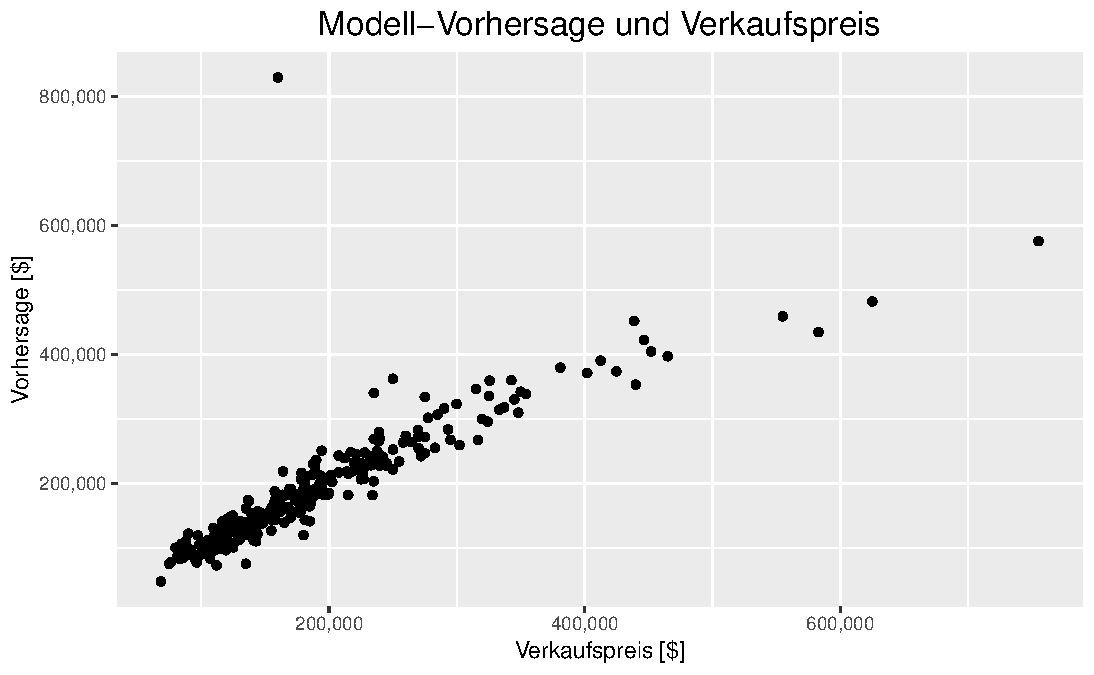
\includegraphics[width=\textwidth, keepaspectratio]{figures/simple_model}
	\end{figure}
	
\end{frame}


\begin{frame}{Interpretierbare Koeffizienten}
	
	\begin{Large}{Nachteil unstandardisierter Regressionskoeffizienten}\end{Large}
	
	  \begin{itemize}
		\item Von den Maßeinheiten für X und Y abhängig
		\item Daher schlechtere Vergleichbarkeit
	  \end{itemize}
	 
	\begin{Large}{Lösung: Standardisierte Koeffizienten}\end{Large}
	
\end{frame}

\begin{frame}{Beta-Koeffizienten im Vergleich}
	
	\begin{figure}
		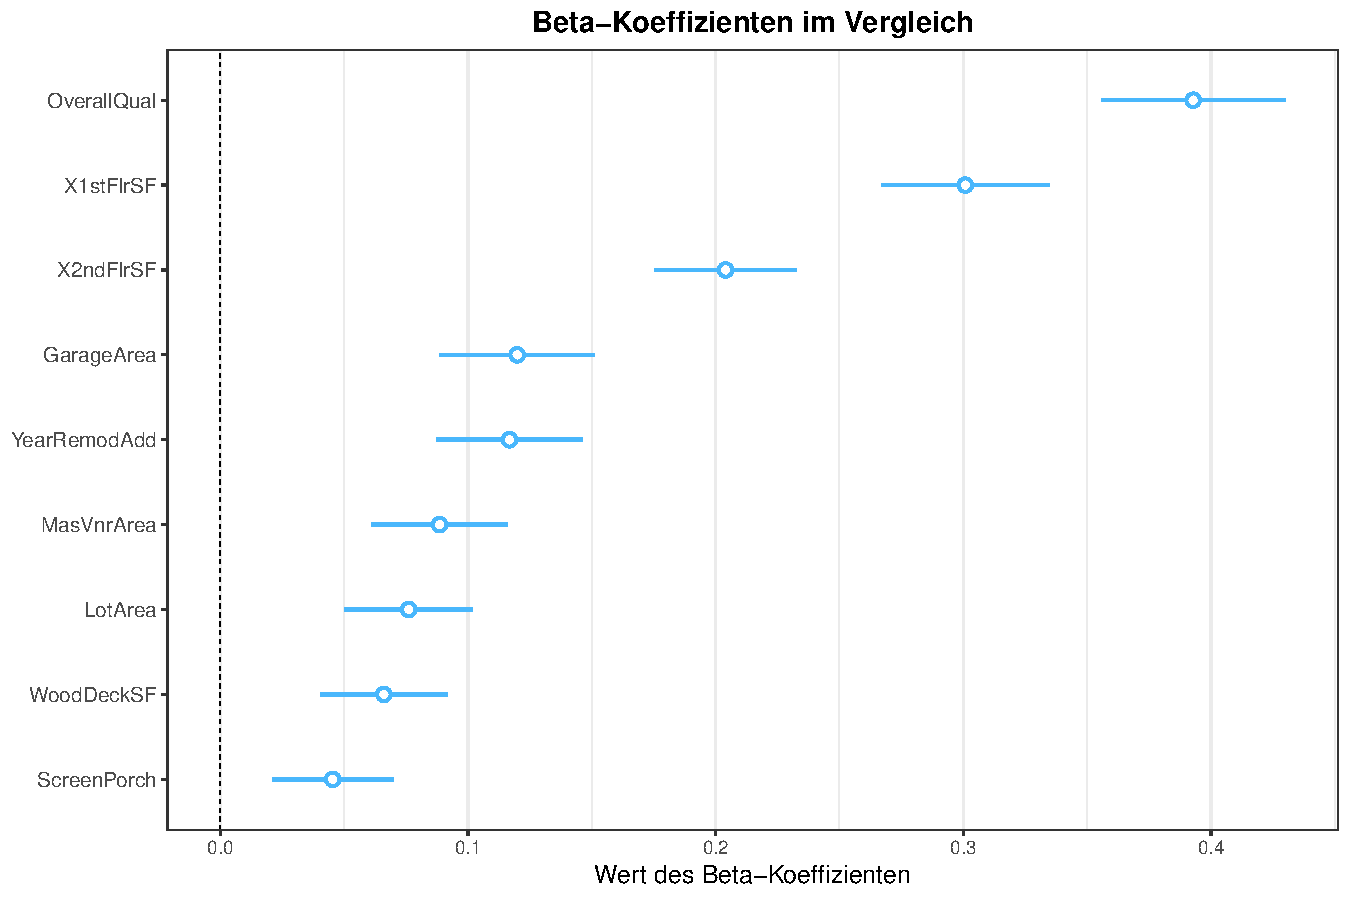
\includegraphics[width=\textwidth, keepaspectratio]{figures/beta_koeffizienten}
	\end{figure}

\end{frame}


\section{Regularisierung}

\begin{frame}{Problemstellung I}
        \begin{figure}
            \centering
                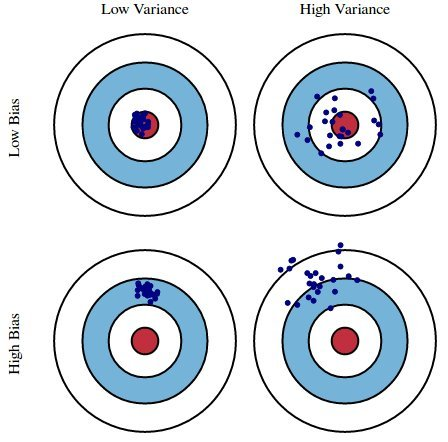
\includegraphics[width=0.5\textwidth, keepaspectratio]{figures/bias-and-variance.jpg}
            \caption{Quelle: kdnuggets.com}
         \end{figure}
    
        \begin{itemize}
            \item Bias- Variance Tradeoff
            \item OLS Schätzer ist "unbiased" aber kann große Varianz haben
        \end{itemize}
    
\end{frame}

\begin{frame}{Problemstellung II}
        
        \begin{Large}{Wann tritt große Varianz auf?}\end{Large}
        
        \begin{itemize}
            \item Wenn die Prediktoren hohe Korrelation aufweisen
            \item Bei vielen Prediktoren. Wenn die Anzahl Prediktoren nahe bei Anzahl der Beobachtungen geht die Varianz gegen unendlich.
        \end{itemize}
    
\end{frame}

\begin{frame}{Lösung}

    \begin{Large}{Verringerung der Varianz auf Kosten des Bias}\end{Large}

        \begin{figure}
            \centering
            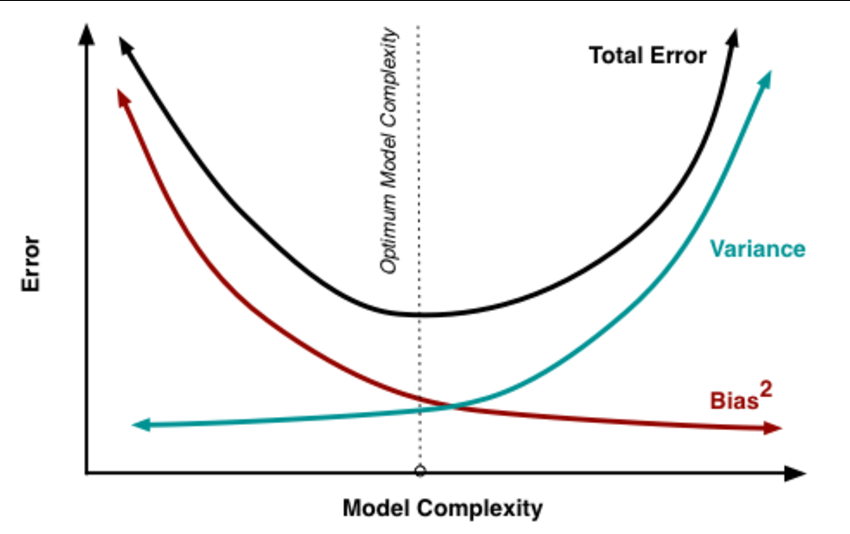
\includegraphics[width=0.9\textwidth]{figures/complexity_error.png}
            \caption{Quelle: researchgate.net}
        \end{figure}
        
\end{frame}

\begin{frame}{Ridge Regression}
	
    \begin{equation*}
        L_{ridge}(\hat{\beta})=\sum_{i=1}^{n}(y_{i}-x_{i}'\hat{\beta})^2+\lambda\sum_{j=1}^{m}\hat{\beta}_{j}^2=||y-X\hat{\beta}||^2+\lambda||\hat{\beta}||^2
    \end{equation*}
    Man erhält für jeden Parameter $\lambda$ ein set von Schätzern $\hat{\beta}$.
    Falls $\lambda \Rightarrow 0$, dann $\hat{\beta}_{ridge} \Rightarrow \hat{\beta}_{OLS}$
    Frage: wie wird der Regularisierungs- Parameter gewählt?
    \begin{itemize}
        \item Crossvalidierung (hier)
        \item Minimierung eines weiteren Informationskriteriums (AIC, BIC etc.)
    \end{itemize}
    
\end{frame}

\begin{frame}{Ridge Regression: Crossvalidierung}

    \begin{figure}
        \centering
        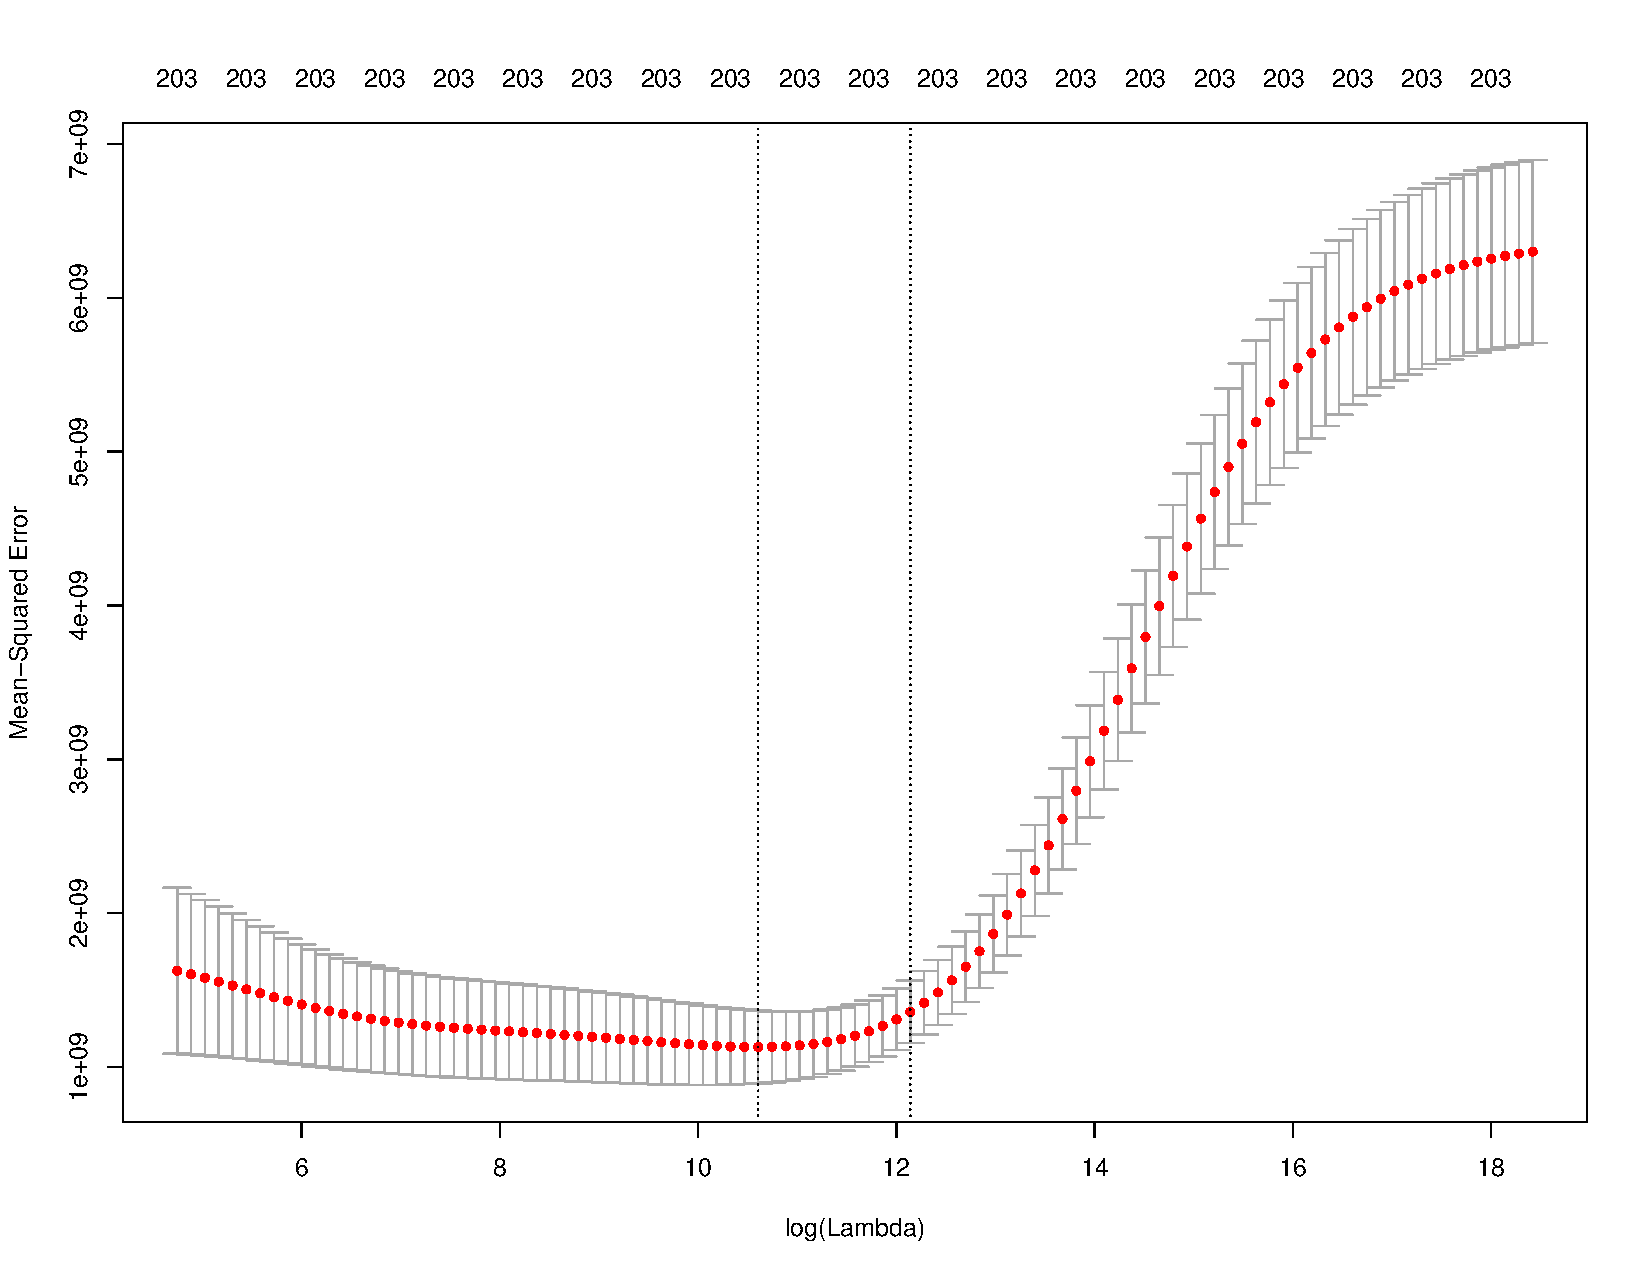
\includegraphics[width=0.8\textwidth, keepaspectratio]{figures/ridge_tuning.pdf}
        \caption{Lambda Tuning}
    \end{figure}
    
\end{frame}

\begin{frame}{Lasso Regression}

    \begin{Large}{Lasso, or Least Absolute Shrinkage and Selection Operator}\end{Large}
    
    Ridge: L2 Penalty
    \newline
    Lasso: L1 Penalty
	
	\begin{equation*}
	L_{lasso}(\hat{\beta})=\sum_{i=1}^{n}(y_{i}-x_{i}'\hat{\beta})^2+\lambda\sum_{j=1}^{m}|\hat{\beta}_{j}|=||y-X\hat{\beta}||^2+\lambda||\hat{\beta}||_{1}
	\end{equation*}
    Tuning:
	\begin{itemize}
		\item Crossvalidierung (hier)
		\item Minimierung eines weiteren Informationskriteriums (AIC, BCI etc.)
	\end{itemize}
	
\end{frame}

\begin{frame}{Lasso Regression: Crossvalidierung}
	
	\begin{figure}
		\centering
		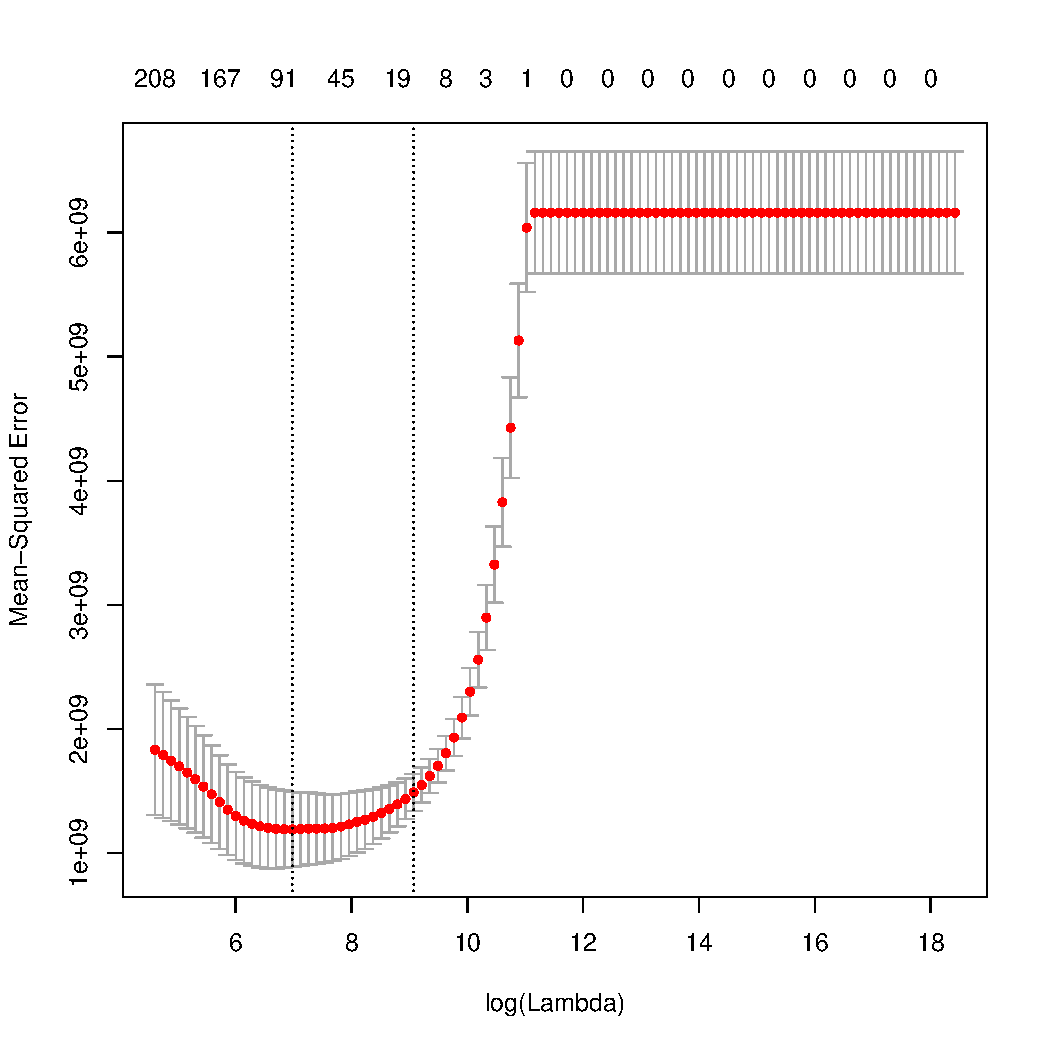
\includegraphics[height=.7\textheight]{figures/lasso_cv.pdf}
		\caption{Lambda Tuning}
	\end{figure}
	
\end{frame}


\begin{frame}{Lasso Regression: Koeffizienten}
	
	\begin{figure}
		\centering
		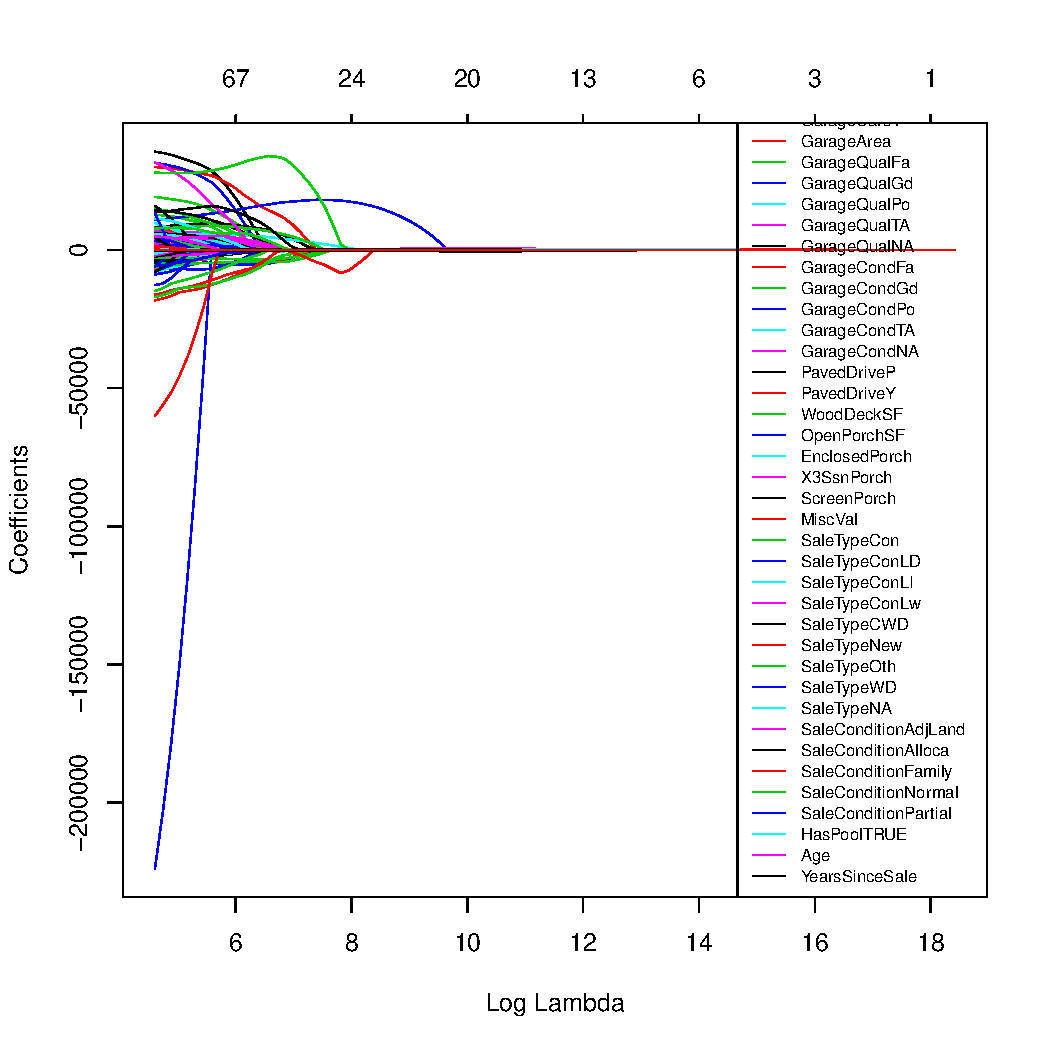
\includegraphics[height=.7\textheight]{figures/lasso_coeff.pdf}
		\caption{Lambda Tuning}
	\end{figure}
	
\end{frame}



\begin{frame}{Vergleich der Modelle}
\begin{table}[ht]
\centering
\begin{tabular}{rlll}
  \hline
 & Modelle & R$^2$ & MAD \\ 
  \hline
   & OLS & 0.933 & 20117 \\ 
   & Ridge & 0.903 & 19624 \\ 
   & Lasso & 0.904 & 30010\\ 
   \hline
\end{tabular}
\end{table}

\end{frame}

\begin{frame}{Anmerkungen}

    \begin{itemize}
        \item Feature Selection mit Lasso möglich, mit Ridge nicht.
        \item Beide Methoden können gut mit Multikolinearität umgehen (Ridge: korrelierte Koeffizienten sind ähnlich groß, Lasso: ein Koeffizient groß, die von korrelierten Prediktoren sind nahe bei Null)
    \end{itemize}
    Verallgemeinerte Regularisierung linearer Modelle: Elastic Net
    \begin{equation*}
        L_{enet}(\hat{\beta})=\frac{\sum_{i=1}^{n}(y_i-x'_i\hat{\beta})^2}{2n}+\lambda(\frac{1-\alpha}{2}\sum_{j=1}^{m}\hat{\beta}_j^2+\alpha\sum_{j=1}^{m}|\hat{\beta}_j|)
    \end{equation*}
    
\end{frame}

\begin{frame}{Fragen und Diskussion}
	\begin{LARGE}
		\begin{center}
			Vielen Dank für\\eure Aufmerksamkeit!
		\end{center}
	\end{LARGE}
\end{frame}

\end{document}
